\section{Circuit description}
\label{sec:analysis}

\begin{figure}[h] \centering
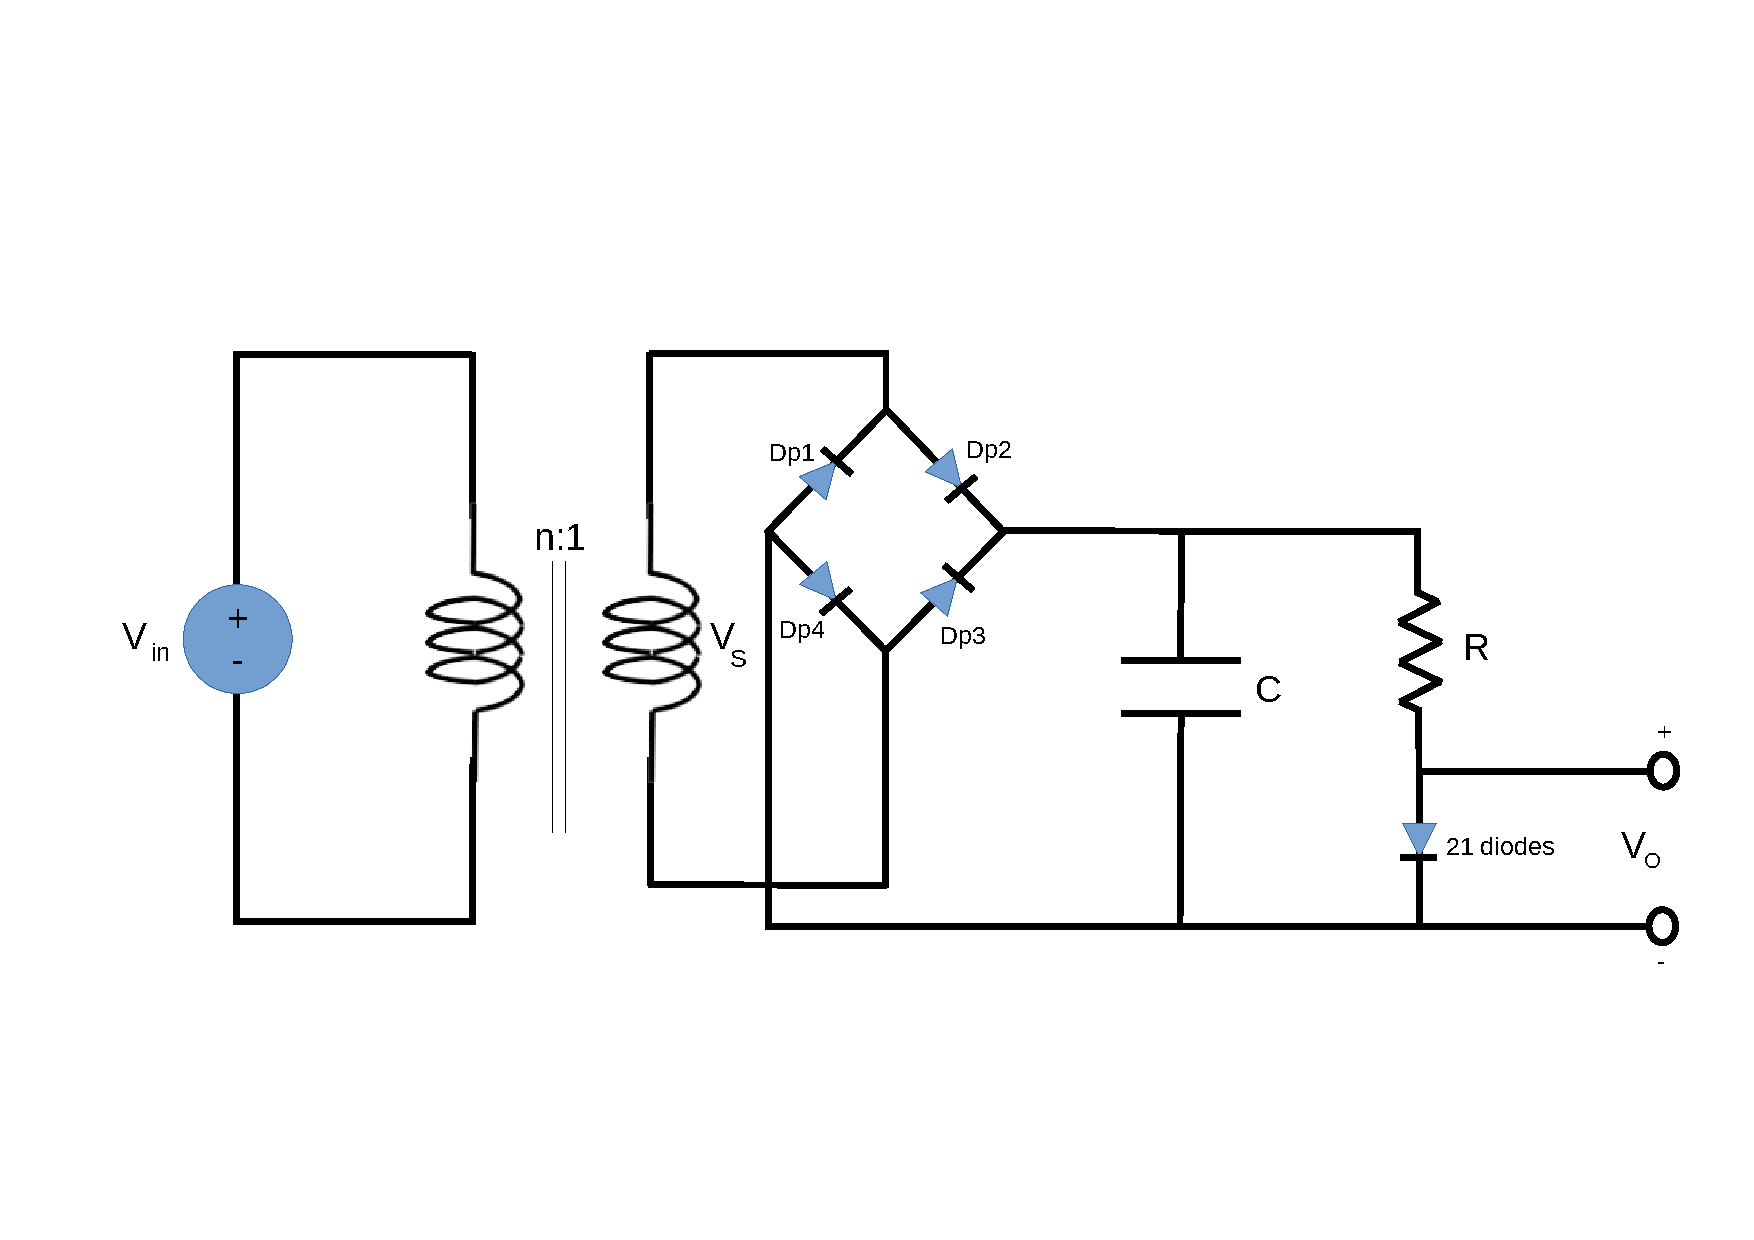
\includegraphics[width=1\linewidth]{../figlib/lab3.pdf}
\caption{Circuit to be analysed in this report.}
\label{fig:lab3}
\end{figure}


In this section, we will descrive the circuit shown in Figure \ref{fig:lab3}. In our configuration we use a transformer that has a ratio $15.54:1$. 
Connected to the transformer, we use a full-wave bridge rectifier, using four diodes, and a capacitor connected in parallel with the rectifier. 
These two elements make the envelope detector. Then we connect in parallel with this circuit a series of 21 diodes and one resistor, consisting on a voltage regulator. 
In the following table we present the values to the the various components and parameters.

\begin{table}[h]
  \centering
  \begin{tabular}{|l|r|}
    \hline    
    {\bf Name} & {\bf Value [{$\Omega$} or V or Hz or F]} \\ \hline
    \input{../mat/Circuit.tex}
  \end{tabular}
  \caption{Values of the various components and parameters}
  \label{tab:Circuit}
\end{table}

\newpage
\section{Circuit Analysis}

In the following section we present the theoretical and simulation analysis, using Octave and Ngspice, respectively, comparing each other. To start with we will take a look at the voltage output, $V_S$,
from the transformer. In both analysis the results obtained naturally don't differ, so we will just present one graph, in this case, produced by Octave.

\begin{figure}[h] \centering
\includegraphics[width=0.4\linewidth]{vs.eps}
\caption{Results for $V_S$.}
\label{fig:1}
\end{figure}

Moving on to the output voltage from the envelope detector we can also expect not having the same results cause ngspice use complex methods and we are using the $V_{ON}$ aproximation.
Dispite that we can observe that the differences are small, meaning that the ideal diode model works "just fine". 
\vspace{-2cm}
\begin{figure}[h!]
            \centering
            \subfigure[]{\includegraphics[width=0.49\textwidth]{Vc.eps}} 
            \subfigure[]{\includegraphics[width=0.40\textwidth]{envdec.pdf}} 
            \caption{a) Voltage in envelope detector using octave b) Voltage in envelope detector using ngspice}
            \label{fig:2}
\end{figure}

In both plots we chose to neglect the first period since in ngspice in that time the circuit was not stable which would result in a bad calculation of the average values. 

Lastly, we had to analyse the output voltage from the voltage regulator. In this last analysis we were also expecting some diferences between both theoretical and simulation results, but in this case we
expected lower differences due to the usage of a more accurate model which consists of solving non-linear equations using Newton-Raphson method.  

\begin{figure}[h!]
            \centering
            \subfigure[]{\includegraphics[width=0.49\textwidth]{vo.eps}} 
            \subfigure[]{\includegraphics[width=0.40\textwidth]{volreg.pdf}} 
            \caption{a) Voltage in voltage regulator using octave b) Voltage in voltage regulator using ngspice}
            \label{fig:3}
\end{figure}

\section{Discussion of various tests and final results}

In this section, we are going to discuss about some tests that were elaborated during the laboratory preparation which led to the final circuit (presented in the section \ref{sec:analysis}). 
To compare the different configurations and to reach the best one we were based on the merit calculation. That is given by the formula: 

\begin{equation}
M=\frac{1}{(cost\cdot(ripple(V_o)+average(V_{o}-12)+10^{-6}))}
\end{equation}
\\

Being the cost equal to the sum of the cost of the capacitor, diodes and resistors.
The cost of the of the resistors equal to 1 monetary unit (MU) per Ohm, the cost of the diodes 0.1 MU per diode and the cost of the capacitor is 1 MU per {\textmu}F.

By the formula it's crucial to not only have voltage output close to 12V and with low ripple, but also reduce as much as we can the cost. 
\par Firstly, we tryed to use an half-wave rectifier but we had to spend too much money on resistance and capacitance to reduce the high ripple due to the presence of only an half-wave rectifier,
so from the start we had it clear that we needed to use a full-wave rectifier since the cost of three more diodes was definitely better than the waste on the other two components.
Then we established the configuration presented in this assignment and the final one came from the alteration of the values of the resistance and capacitance and the number of diodes in the regulator. 
\par So from all the configurations that were made we conclude that:
\begin{itemize}
\item High resistance and high capacitance lead to very low ripple and the average very close to 12V, but it was too expensive so we couldn't achieve a good merit;
\item Low resistance and low capacitance are cheap in terms of the cost, but in terms of the output voltage there is too high ripple eventhough the average stays around 12V so the merit was not that good;
\item If we spend a certain amount of money, the merit was not so good if we spend much more in resistance than in capacitance, and vice-versa. So we should not invest too much in only one of them;
\end{itemize}

After all the testing we can now look back at our best configuration and its results. 
\vspace{-2cm}
\begin{figure}[h!]
            \centering
            \subfigure[]{\includegraphics[width=0.49\textwidth]{vo_dif.eps}} 
            \subfigure[]{\includegraphics[width=0.40\textwidth]{final.pdf}} 
            \caption{a)Deviation from 12V using octave b)Deviation from 12V using ngspice}
            \label{fig:4}
\end{figure}

As you can see in the graphs we have a small ripple and the average is close to 12V (can be seen in the nexts tables).
Also they present similar results but for the reasons mencioned in section \ref{sec:analysis} (these plots are pretty closed to the previous ones, only deviated vertically from 12V).

The average values of the output are presented in the tables \ref{tab:2} and \ref{tab:3}. 

\begin{table}[!htb]
	\begin{minipage}{.5\linewidth}
	\centering
	\begin{tabular}{ll}
	{\bf Name} & {\bf Value [V]} \\ \hline
	\input{../mat/Average.tex}
	\end{tabular}
	\caption{Average using Octave.}
	\label{tab:2}
  	\end{minipage}
  	\hfill
	\begin{minipage}{.5\linewidth}
	\centering
  	\begin{tabular}{ll}
   	{\bf Name} & {\bf Value [V]} \\ \hline
   	@c1[i] & 0.000000e+00\\ \hline
@gb[i] & -2.08664e-04\\ \hline
@r1[i] & 1.992363e-04\\ \hline
@r2[i] & 2.086637e-04\\ \hline
@r3[i] & -9.42740e-06\\ \hline
@r4[i] & 1.200363e-03\\ \hline
@r5[i] & -2.08664e-04\\ \hline
@r6[i] & 1.001127e-03\\ \hline
@r7[i] & 1.001127e-03\\ \hline
v(1) & 5.195199e+00\\ \hline
v(2) & 4.989875e+00\\ \hline
v(3) & 4.556619e+00\\ \hline
v(5) & 5.019215e+00\\ \hline
v(6) & 5.659286e+00\\ \hline
v(7) & -2.01262e+00\\ \hline
v(8) & -2.01262e+00\\ \hline
v(9) & -3.01963e+00\\ \hline

	\end{tabular}
	\caption{Average using Ngspice.}
	\label{tab:3}
	\end{minipage}
\end{table}

The ripple values of the output are presented in the tables \ref{tab:4} and \ref{tab:5}.

\begin{table}[!htb]
	\begin{minipage}{.5\linewidth}
	\centering
	\begin{tabular}{ll}
	{\bf Name} & {\bf Value [V]} \\ \hline
	\input{../mat/ripple.tex}
	\end{tabular}
	\caption{Ripple using Octave.}
	\label{tab:4}
  	\end{minipage}
  	\hfill
	\begin{minipage}{.5\linewidth}
	\centering
  	\begin{tabular}{ll}
   	{\bf Name} & {\bf Value [V]} \\ \hline
   	@gb[i] & 1.053111e-17\\ \hline
@r1[i] & -1.00553e-17\\ \hline
@r2[i] & -1.05311e-17\\ \hline
@r3[i] & 4.757942e-19\\ \hline
@r4[i] & 2.124111e-18\\ \hline
@r5[i] & -2.82934e-03\\ \hline
@r6[i] & 1.734723e-18\\ \hline
@r7[i] & 1.830908e-18\\ \hline
v(1) & 0.000000e+00\\ \hline
v(2) & 1.036259e-14\\ \hline
v(3) & 3.222868e-14\\ \hline
v(5) & 8.881784e-15\\ \hline
v(6) & 8.678914e+00\\ \hline
v(7) & -3.48740e-15\\ \hline
v(8) & -3.48740e-15\\ \hline
v(9) & -5.32907e-15\\ \hline

	\end{tabular}
	\caption{Ripple using Ngspice.}
	\label{tab:5}
	\end{minipage}
\end{table}

The average and ripple values are close between each analysis which means that the methods used work good dispite the differences.

In the next table we present the cost and the merit obtained using Ngspice. 
\vspace{1cm}
\begin{table}[h]
  \centering
  \begin{tabular}{|l|r|}
    \hline    
    {\bf Name} & {\bf Value} \\ \hline
    \input{../mat/table3_tab.tex}
  \end{tabular}
  \caption{Cost and merit.}
  \label{tab:6}
\end{table}








